\documentclass[a4paper]{article}
\usepackage[utf8]{inputenc}
\usepackage[russian,english]{babel}
\usepackage[T2A]{fontenc}
\usepackage[left=10mm, top=20mm, right=18mm, bottom=15mm, footskip=10mm]{geometry}
\usepackage{indentfirst}
\usepackage{amsmath,amssymb}
\usepackage[italicdiff]{physics}
\usepackage{graphicx}
\graphicspath{{images/}}
\DeclareGraphicsExtensions{.pdf,.png,.jpg}
\usepackage{wrapfig}
\usepackage{pgfplots}

\usepackage{caption}
\captionsetup[figure]{name=Рисунок}
\captionsetup[table]{name=Таблица}

\title{\underline{Лабораторные работы 1.3.1 и 1.3.2}}
\author{Старстин Александр, Б01-401}


\begin{document}

\maketitle
\newpage
\begin{figure}[!ht]
\newpage
    \centering
    \textbf{Определение модуля Юнга на основе исследования деформации растяжения.}\\
    \textbf{Определение модуля кручения.}
\end{figure}

\section{Аннотация}
    \par \textbf{Цель работы:} Экспериментально получить зависимость между напряжением и деформацией для одностороннего растяжения; по результатам эксперимента вычислить модуль Юнга. \\

    \par \textbf{В работе используются:} Прибор Лермантова, проволока из исследуемого материала, зрительная трубка со шкалой, набор грузов, микрометр, рулетка или линейка. Проволка из исследуемого материала,
грузы, секундомер, микрометр, рулетка, линйка.

\section{Определение модуля Юнга по измерению растяжения проволки}

\subsection{Теоретические сведения}

Связь между удлинением проволки $\Delta l$ и силой $P$, вызывающей это удлинение, выражается законом Гука:

\begin{equation}\label{lermantov}
    \frac{P}{S}=E\frac{\Delta l}{l}
\end{equation}

где $l$ - начальная длина проволки, $S$ - её сечение, $E$ - константа, характеризующая упругие свойства материала (модуль Юнга).\\\\

Опыт проводится на приборе Лермантова (рис. прибора см. ниже).

\begin{figure}[!ht]
    \centering
    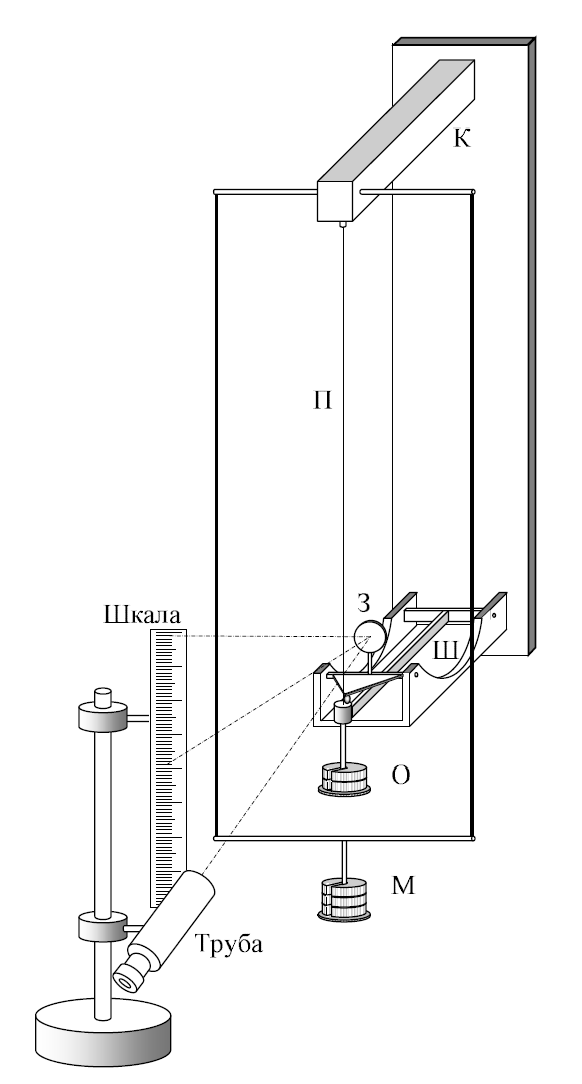
\includegraphics[scale=0.4]{lermantov.png}
    \caption{Прибор Лермантова}
\end{figure}

\newpage
\subsection{Ход работы}



\subsubsection {Подготовка прибора Лермантова}

Зрительная труба на приборе Лермантова была направлена на зеркальце З так, что в неё было чётко видно отражение шкалы на зеркальце.\\

Формула, связывающая отсчёт по шкале $n$, расстояние от шкалы до зеркала $h$, длину рычага $r$ и удлинение проволки $\Delta l$:

\begin{equation}\label{lermantov}
    {\Delta l}={\Delta n}\frac{r}{2h}
\end{equation}

Значения $r$ и $h$ в опыте:

\begin{table}[h!]
\begin{center}
\begin{tabular}{|c|c|c|c|c|}
\hline
$r$, мм   & $h_1$, cм   & $h_2$, cм   & $\langle h \rangle$, см   & $\sigma_h$, мм      \\ \hline

15   & 1445   & 1445   &1445   &{1}     \\ \hline

\end{tabular}
\caption{Таблица измерений размеров утановки.}
\end{center}
\end{table}

\item $\sigma_{r} = 1$ мм.
\item $\sigma_{h} = 0,1$ cм.\\




\subsubsection {Сечение проволки}

Сечение проволки диаметром $d$ вычисляется по формуле:

\begin{equation}\label{lermantov}
    {S}=\frac{\pi d^2}{4}
\end{equation}

\item Велечина диаметра проволки составляет: ${d} = {0.46} \pm {0.01}$ мм.\\
\item Сечение проволки составляет: ${S} = 0.17$ мм{^2}.\\

\item Погрешность сечения: $\sigma_{S} = {2}{S}\frac{\sigma_{d}}{d} = {0.01}$ мм{^2}.\\



\subsubsection {Длина проволки}

\begin{table}[h!]
\begin{center}
\begin{tabular}{|c|c|c|c|}
\hline
$l_1$, см    & $l_2$, см    & $\langle l \rangle$, см    & $\sigma_l$, см   \\ \hline

177   & 177   &177   &{0.1}      \\ \hline

\end{tabular}
\caption{Таблица измерений длины проволки.}
\end{center}
\end{table}



\subsubsection {Оценка величины максимальной нагрузки}

Во время выполнения работы рабочее напряжение $\sigma$ было {<} {265} H/мм$^2$ (см таблицу с расчётом механического напряжения).
Значит в течение всей работы напряжение не превышало максимальную нагрузку на проволку.

\newpage
\subsubsection {Основные измерения}


\begin{table}[h!]
\begin{center}
\begin{tabular}{|c|c|c|c|c|c|c|c|c|c|c|}
\hline
&$m$, г & $P$, H & $\sigma$, H/мм$^2$ & -> & <- & -> & <- & $\langle \Delta n \rangle$, см & $\langle \Delta l \rangle$, мм & $E * 10^{11}$, Па\\ \hline

1   & 0        & 0    & 0      & 18,0   & 18,0   & 18,0   & 18,0  & 0     & 0     & -     \\ \hline
2   & 245,8    & 2,4  & 14,0   & 21,1   & 21,1   & 21,1   & 21,0  & 3,1   & 0,16  & 1,562         \\ \hline
3   & 491,4    & 4,8  & 28,2   & 24,0   & 24,0   & 24,0   & 23,9  & 6,0   & 0,31  & 1,612 \\ \hline
4   & 736,7    & 7,2  & 42,4   & 26,7   & 26,6   & 26,7   & 26,6  & 8,7   & 0,45  & 1,666  \\ \hline
5   & 982,2    & 9,6  & 56,5   & 29,4   & 29,3   & 29,4   & 29,3  & 11,4  & 0,60  & 1,666  \\ \hline
6   & 1226,5   & 12,0 & 70,6   & 32,0   & 31,9   & 31,9   & 32,0  & 14,0  & 0,73  & 1,712  \\ \hline
7   & 1471,8   & 14,4 & 84,7   & 34,5   & 34,5   & 34,5   & 34,5  & 16,5  & 0,86  & 1,743   \\ \hline
8   & 1717,3   & 16,8 & 98,8   & 36,9   & 37,1   & 37,0   & 37,1  & 19,0  & 0,99  & 1,767 \\ \hline
9   & 1962,9   & 19,2 & 113,0  & 39,6   & 39,3   & 39,6   & 39,6  & 21,5  & 1,12  & 1,785    \\ \hline
10  & 2209,0   & 21,6 & 127,1  & 42,0   & 41,6   & 42,0   & 42,2  & 24,0  & 1,25  & 1,799  \\ \hline
11  & 2454,6   & 24,0 & 141,2  & 44,4   & 43,9   & 44,3   & 44,3  & 26,2  & 1,34  & 1,865  \\ \hline
12  & 2700,2   & 26,5 & 155,9  & 47,0   & 47,0   & 46,6   & 46,6  & 28,8  & 1,49  & 1,852   \\ \hline

\end{tabular}
\caption{Таблица основных измерений}
\end{center}
\end{table}

\item Среднее $\langle E \rangle = 1,730 * 10^{11}$ Па.\\



\subsubsection {График}

Построим график зависимости нагрузки $m (г)$ от удлинения проволоки $\langle \Delta l \rangle (см)$. Найдем уравнение получившийся прямой по МНК. По наклону прямой определим модуль Юнга.
\\\\

\begin{figure}[!ht]
    \centering
    \begin{tikzpicture} [hu!]
        \begin{axis}[
        legend pos = north west,
        title  = Зависимость $m$ от $\langle \Delta l \rangle$,
        width  = {360},
        height = {320},
    	ylabel = {$m$, г},
    	xlabel = {$\langle \Delta l \rangle$, см},
    	minor tick num = 4,
        xmin   = {0},
        ymin   = {0},
        xmax   = {1.7},
        ymax   = {3000}
        ]

        \legend{
        	Измерения,
            Наилучшая прямая
        };

        \addplot [blue, mark = *] coordinates{
        	(0, 0) (0.16, 245.8) (0.31, 491.4) (0.45, 736.7) (0.6, 982.2) (0.73, 1226.5) (0.86, 1471.8) (0.99, 1717.3) (1.12, 1962.9) (1.25, 2209.0) (1.34, 2454.6) (1.49, 2700.2)
        };



        \addplot[dashed, draw = red]{1765.3 * x};

        \end{axis}
    \end{tikzpicture}
\end{figure}

Расчёт по МНК:\\
\item $k = \frac{\langle m {\langle \Delta l \rangle} \rangle } {{\langle {\langle \Delta l \rangle} ^ 2 \rangle}} = {1765,3}$ г/мм.\\

\\
\item Расчёт модуля юнга через график: $E = k * \frac{{g} * {\langle l \rangle}}{S} = 1,801 * 10 ^ {11}$ Па.

\subsubsection {Погрешность измерения модуля юнга.}
Случайной погрешностью в данном можно пренебречь, тк она мала. Тогда, будем учитывать приборную погрешность:\\

\item Масса: $\sigma_{m}$ = 0,03 г  {   и   }  $\overline{m}$ = 1349,87 г.\\
\item Сечение: $\sigma_{S}$ = 0,01 мм$^2$  {   и   }    $\overline{S}$ = 0,17 мм$^2$.\\
\item Длина: $\sigma_{l}$ = 0,1 см  {   и   }    $\overline{l}$ = 177,0 см.\\
\item Удлинение: $\sigma_{\Delta l}$ = 0.05 мм  {   и   }    $\overline{\Delta l}$ = 0,78 мм.\\

\item $\sigma_{\Delta l} = {\overline{\Delta l}} * \sqrt{(\frac{\sigma_{r}}{r})^2 + (\frac{\sigma_{h}}{h})^2 + (\frac{\sigma_{\Delta l}}{\overline{\Delta l}})^2}$ = 0.05 мм.\\\\

\item Погрешность $\overline{E}:$ {       } $\sigma_{E} = E * \sqrt{({\frac{\sigma_{m}}{\overline{m}})^2 + ({\frac{\sigma_{S}}{\overline{S}})^2 + (\frac{\sigma_{l}}{\overline{l}})^2 + (\frac{\sigma_{\Delta l}}{\overline{\Delta l}})^2}$ = 0.15 * 10$^{11}$ Па.\\

\item Тогда результат измерений Модуля Юнга: ${E} = ({1,73} \pm {0,15}) * 10^{11}$ Па.\\




\newpage





\section{Измерение модуля кручения и модуля сдвига динамическим способом}

    \par \textbf{Цель работы:} Измерение углов закручивания в зависимости от приложенного момента сил, определение модулей кручения и сдвига для проволки по измерениям периодов крутильных колебаний подвешенного на ней маятника.\\

    \par \textbf{В работе используются:} Проволка из исследуемого материала,
    грузы, секундомер, микрометр, рулетка, линейка.\\

\subsection {Теоретические сведения}

    Модуль кручения $f$ связан с модулем сдвига $G$ соотношением:
    \begin{equation}
        G=\frac{2l}{\pi R^{4}}f
    \end{equation}
    где $R$ - радиус крутящегося цилиндра.\\


    Период кoлебаний системы связан с расстоянием $r$ от оси вращения до грузов и
    моментом инерции стержня $I_0$ следующим образом:

    \begin{equation}
        T^2=(2\pi)^2\frac{I}{f}=(2\pi)^2\frac{I_0}{f}+(2\pi)^2\frac{(m_1+m_2)}{f}r^2
    \end{equation}

    Эта зависимость верна для незатухающих колебаний. Из неё, найдя $f$, получим $G$.\\

    Схема установки:
    \begin{figure}[!ht]
        \centering
        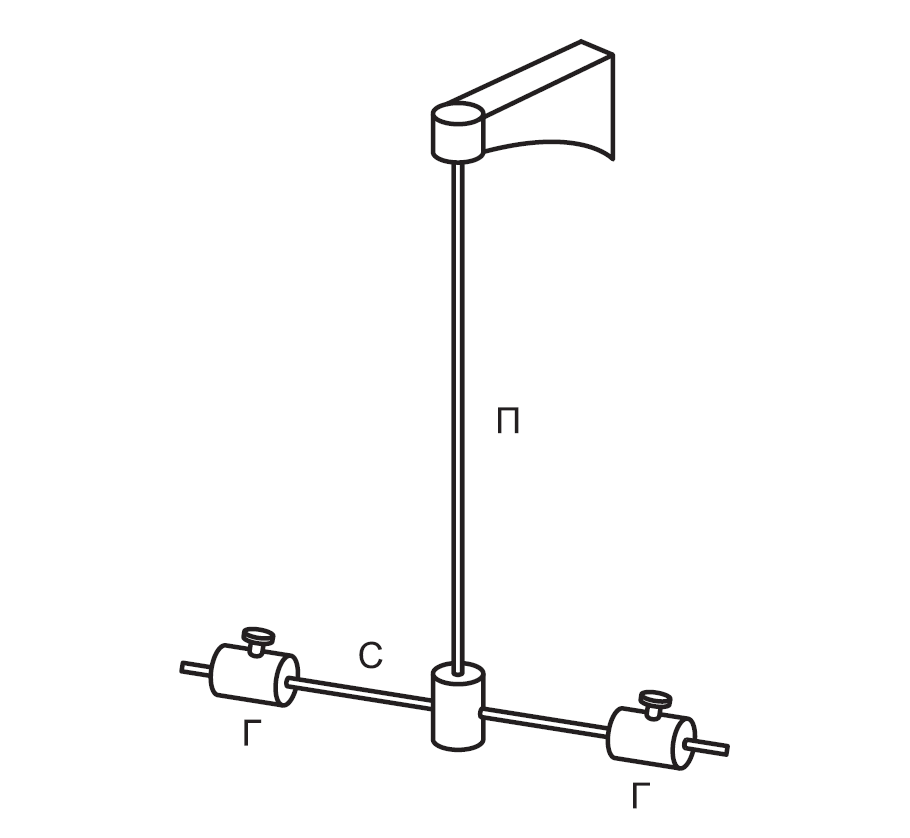
\includegraphics[scale=0.4]{cruchenie.png}
        \caption{Крутильная установка.}
    \end{figure}

\subsection {Ход работы}

\subsubsection {Проверка того, что при разных амплитудах периоды крутильных колебаний одинаковые.}

    \begin{table}[h!]
    \begin{center}
    \begin{tabular}{|c|c|c|c|}
    \hline
    $\varphi$, \circ    & Время $t$, с    & Количество колебаний $N$    & Период $T$, с   \\ \hline

    15   & 72,07   & 20  & 3.64      \\ \hline
    15   & 72,07   & 20  & 3.64      \\ \hline
    25   & 72,07   & 20  & 3.64      \\ \hline
    25   & 72,04   & 20  & 3.62      \\ \hline

    \end{tabular}
    \caption{Таблица измерений периодов при разных ампилитудах }
    \end{center}
    \end{table}

    Все периоды можно считать равными. Значит, при разных амплитудах периоды колебаний одинаковые и, следовательно, период колебаний не зависит от начальной амплитуды.

\newpage

\subsubsection {Проверка того, что колебания можно считать незатухающими.}

    Измерим амплитуду колебаний в начале колебаний и через 50 периодов:

    \begin{table}[h!]
    \begin{center}
    \begin{tabular}{|c|c|}
    \hline
    Количество прошедших колебаний $N$    & $\varphi$, \circ   \\ \hline

    1    & 15         \\ \hline
    50   & 12,5       \\ \hline

    \end{tabular}
    \caption{Таблица измерений ампилитуды колебаний}
    \end{center}
    \end{table}

    Спустя 50 колебаний ампилитуда колебаний изменилась в $\frac{15}{12,5}$ = 1,2 раза. Тк амплитуда за 50 колебаний уменьшается меньше, чем в два раза (1,2 < 2), то колебания можно считать не затухающими.

\subsubsection {Измерение модуля кручения и вычисление модуля сдвига.}
    Установим грузы на одинаковом расстоянии $r$ от оси вращения проволки до центра масс каждого груза. Меняя $r$, будем считать для каждого случая период колебаний:

    \begin{table}[h!]
    \begin{center}
    \begin{tabular}{|c|c|c|c|}
    \hline

    $r$, см    & $T1$, c  & $T2$, c   & $\overline{T}$, c  \\ \hline

    12,0    & 3,60   & 3,60   & 3,60         \\ \hline
    13,0    & 3,82   & 3,82   & 3,82         \\ \hline
    14,0    & 4,05   & 4,05   & 4,05         \\ \hline
    15,0    & 4,31   & 4,31   & 4,31         \\ \hline
    16,0    & 4,54   & 4,54   & 4,54         \\ \hline
    17,0    & 4,79   & 4,79   & 4,79         \\ \hline
    18,0    & 5,02   & 5,02   & 5,02         \\ \hline

    \end{tabular}
    \caption{Таблица измерений периодов колебаний при разных $r$}
    \end{center}
    \end{table}

    Из формулы (5) видно, что $T^2$ зависит линейно от $r^2$. Значит, зная массы грузов, можно найти из графика зависимости уголовой коэффициента наклона прямой и из него найти модуль кручения.

    Массы грузов:

    \begin{table}[h!]
    \begin{center}
    \begin{tabular}{|c|c|c|}
    \hline

    $m1$, г    & $m2$, г  & $m1+m2$, г    \\ \hline

    202,5    & 204,9   & 407,4            \\ \hline


    \end{tabular}
    \caption{Таблица измерений масс грузов}
    \end{center}
    \end{table}

    Точки для графика:

    \begin{table}[h!]
    \begin{center}
    \begin{tabular}{|c|c|c|}
    \hline

    $r^$, см$^2$    & $T^2$, с$^2$      \\ \hline

    144,0    & 12,96              \\ \hline
    169,0    & 14,59              \\ \hline
    196,0    & 16,40              \\ \hline
    225,0    & 18,58              \\ \hline
    256,0    & 20,61              \\ \hline
    289,0    & 22,94              \\ \hline
    324,0    & 25,20              \\ \hline

    \end{tabular}
    \caption{Таблица измерений масс грузов}
    \end{center}
    \end{table}

    Посторим график и наилучшую прямую для него по МНК:

    \newpage

    \begin{figure}[!ht]
        \centering
        \begin{tikzpicture} [hu!]
            \begin{axis}[
            legend pos = north west,
            title  = Зависимость $T^2$ от $r^2$,
            width  = {400},
            height = {350},
        	ylabel = {$T^2$, с$^2$},
        	xlabel = {$r^2$, см$^2$},
        	minor tick num = 4,
            xmin   = {120},
            ymin   = {10},
            xmax   = {360},
            ymax   = {30}
            ]

            \legend{
            	Измерения,
                Наилучшая прямая
            };

            \addplot [blue, mark = *] coordinates{
            	(144.0, 12.96) (169.0, 14.59) (196.0, 16.40) (225.0, 18.58) (256.0, 20.61) (289.0, 22.94) (324.0, 25.20)
            };

            \addplot [dashed, draw = red] coordinates{
            	(144.0, 12.90) (169.0, 14.62) (196.0, 16.48) (225.0, 18.48) (256.0, 20.61) (289.0, 22.88) (324.0, 25.29) (120.0, 11.24) (360.0, 27.77)
            };

            \end{axis}
        \end{tikzpicture}
    \end{figure}

    Расчёты по МНК:\\

    \item $a = \frac{\langle T^2 r^2 \rangle - \langle T^2 \rangle \langle r^2 \rangle}{\langle r^4 \rangle - (\langle r^2 \rangle)^2} = 0,068868$ c$^2$/см$^2$ $= 688,68$ c$^2$/м$^2$\\
    \item $b = \langle T^2 \rangle - a * \langle r^2 \rangle = 2,98$ c$^2$\\
    \item Наилучшая прямая: $T^2 = a * r^2 + b$\\

    Выразим можуль кручения $f$ через $a$:

    \begin{equation}
        f = {4 \pi^2} * \frac{2(m1+m2)}{a}
    \end{equation}

    \item Тогда $f = 4,67 * 10^{-2}$ H*м.\\

    Найдём длину проволки:

    \item $l = 173$ см.\\

    \newpage

    Найдём диаметр и радиус проволки:
    \begin{table}[h!]
    \begin{center}
    \begin{tabular}{|c|c|}
    \hline

    Номер измерения    & $d$, мм      \\ \hline

    1     & 1.56              \\ \hline
    2     & 1.55              \\ \hline
    3     & 1.56              \\ \hline
    4     & 1.57              \\ \hline
    5     & 1.55              \\ \hline
    6     & 1.55              \\ \hline
    7     & 1.56              \\ \hline
    8     & 1.57              \\ \hline
    9     & 1.56              \\ \hline
    10    & 1.56              \\ \hline

    \end{tabular}
    \caption{Таблица измерений диаметра проволки}
    \end{center}
    \end{table}

    \item Средний диаметр $\overline{d} = 1,56$ мм.
    \item Средний радиус  $\overline{R} = 0,78$ мм.\\


    Тогда по формуде (4) модуль сдвиг: $G = 1,39 * 10^{11}$ Па.






\subsubsection {Погрешности.}
    Случайной погрешностью в данном можно пренебречь, тк она мала. Тогда, будем учитывать приборную погрешность:\\

    \item Период: $\sigma_{T}$ = 0,03 c.
    \item Расстояние: $\sigma_{r}$ = 0,1 см.
    \item Масса: $\sigma_{m}$ = 0,3 г.
    \item Длина: $\sigma_{l}$ = 0,2 см.
    \item Радиус: $\sigma_{R}$ = 0,01 мм.

    \item Погрешность G: $\sigma_{G} = G * \sqrt{({\frac{\sigma_{m}}{\overline{m}})^2 + ({\frac{\sigma_{l}}{\overline{l}})^2 + (\frac{\sigma_{R}}{\overline{R}})^2}$ = 0.02 * 10$^{11}$ Па.\\

    \item Тогда результат измерений модуля сдвига: ${G} = ({1,39} \pm {0.02}) * 10^{11}$ Па.\\






\section{Вывод}

    \par Измерен модуль Юнга с помощью прибора Лермантова; результат измерений не сильно отличается от расчёта модуля Юнга из графика наилучшей прямой; погрешность измерения приемлимая, что говорит о хорошей точности измерений.

    \par Измерены модули кручения и сдвига с помощью крутильных колебаний; погрешность измерения приемлимая, что говорит о хорошей точности измерений.


\end{document}
